\chapter{Integration}
\label{chap:Integration}
This chapter provides an in-depth explanation of how the described methods were implemented into the larger \acrshort{xgee} codebase.

\section{System Overview and Workflow}
\label{sec:system_overview}

\acrshort{xgee} is a web-based graphical model editor that utilizes an editor model to define editors for ecore models in a model-driven approach, enabling visualization and interaction. The editor model supports the model-driven definition of editors for ecore models, incorporating both visualization and interaction \cite{waldvogel_annighoefer_models_2024}.

\acrshort{xgee}'s visualization verification is implemented as a modification to the main editor, mostly within the \textit{detector.py} and \textit{diagram\_tokenization\_orchestrator.py} files.
For the verification process to function correctly, a screenshot of the entire screen is preprocessed to isolate the relevant portions of \acrshort{xgee}'s editor window by removing elements like the browser \acrshort{ui} and background grid. During the tokenization step, the positions, dimensions and contents of edges, vertices, and text are detected and stored. This data is subsequently used in the syntactical analysis to identify inconsistencies in parent-child relationships between tokens. (Syntax in this context means the positioning rules of vertices, edges and text labels defined in the editor model.)\\
A new model is then instantiated based on the detected tokens and the visualization model. This model is compared to the original and any discrepancies are highlighted through both graphical and textual user interfaces.\\
Edge, vertex, and text detections occur during the tokenization phase of the verification pipeline. In the original integration, each detection algorithm was implemented as a class within the \textit{detector.py} file, while their execution was managed by the \textit{diagram\_tokenization\_orchestrator.py} file, which determined the order and process of the tokenization. This structure is retained and extended in the new implementation.

\section{Edge Detection Integration}
The integration of the new edge detection algorithm into \acrshort{xgee} is simplified by its use of the already existing interface for inputs and outputs. This approach ensures that the system remains modular and scalable.\\
To implement the new functionality, the algorithm is divided into sections, each expressed as an individual function in the code. These functions are appended to the edge detection class, maintaining modularity and readability. By ensuring the edge detection operates with the same input (screenshots) and provides the same output (\acrshort{opencv} polylines) as the original method, the new implementation can be integrated without requiring large changes to the existing codebase.\\
The \textit{diagram\_tokenization\_orchestrator} queries information such as the stroke width and color from the editor model, which could be used in the future to further generalize the edge detection. It also instantiates an object of the edge detection class, passing the workspace path as an argument to extract data like the intersection template. The polylines are stored using a dedicated data storage function, ensuring subsequent steps proceed smoothly without requiering additional integration effort. 

\section{Vertex Detection Integration}
The integration of a new vertex detection algorithm into \acrshort{xgee}'s codebase required addressing problems such as order-dependent method execution and enabling functions to dynamically share and modify input data at runtime.\\
Previously, a list of vertices for the current editor, generated by the \textit{diagram\_tokenization\_orchestrator}, drove the vertex detection process. The method iterated through this list, performing detection cycles for each vertex type, distinguishing between scalable and non-scalable vertices. However, this static approach proved inadequate in the allocations editor due to overlapping vertices, where detecting the top-level vertex first becomes critical. Furthermore, it was not possible for functions to pass intermediate results, such as detected subtasks, to subsequent functions. This was because the input (a preprocessed screenshot) was initialized at the start of the verification process using the \textit{ImageWrapper} class and remained static throughout.\\
To solve these issues, the new implementation preprocesses the list of editor vertices to ensure vertex detection in the correct hierarchical order and introduces a way for input images to be updated dynamically during runtime.

In the new implementation, the \textit{diagram\_tokenization\_orchestrator} queries vertex attributes such as the filepath, shape, positioning within other vertices and the parent's filepath from the editor model domain. The vertex's position within the list of editor vertices is determined by the presence of the \textit{isPositioningBody} attribute: vertices with this attribute are classified as subvertices, while those without it are considered top-level vertices. Subvertices need to be detected first, as their overlap with parent vertices would otherwise interfere with the reliable detection of those parent vertices.\\
Using these attributes, the list of editor vertices is first sorted, prioritizing subtasks. The \textit{diagram\_tokenization\_orchestrator} then iterates through the sorted list, performing vertex detection for each vertex type. 
To enable the vertex detection function to alter the input of all subsequent iterations of the function, the creation of the \textit{ImageWrapper} object is shifted inside the vertex detection loop. This enables a new \textit{ImageWrapper} Object to be instantiated for every iteration, using the updated image.\\
For subvertices, a new function overlays the detected bounding boxes in the target image with the parent vertex's main color (e.g. the gray of device vertices is used to erase the top-level subtasks). The altered image is then used to instantiate the ImageWrapper, ensuring subsequent stages of vertex detection and verification operate on the updated input. This iterative approach enables precise detection of both subvertices and their parent vertices while simplifying the image progressively.
After all subvertices are processed, almost all remaining vertices can be detected using the methods described in \autoref{sec:vertex_detection}, as the subvertices no longer interfere with the detection process.\\
An alternative approach for resolving overlapping vertices described in \autoref{sec:edge_detection} has been implemented for signal container detection in the allocations editor, facilitating the need to process signal containers seperately using a distinct detection class and seperating them from the other vertices using the \textit{filepath} attribute.\\
Because container vertices are non-scalable, the newly created \textit{ContainerDetector} class inherits from the existing \textit{PortDetector} class (see \autoref{fig:inheritance_diagram}). This inheritance allows the \textit{ContainerDetector} to reutilize the majority of the functionality provided by \textit{PortDetector}, while overriding the \textit{detect\_vertices} function to implement a specialized detection process tailored to container vertices.
\begin{figure}
    \centering
    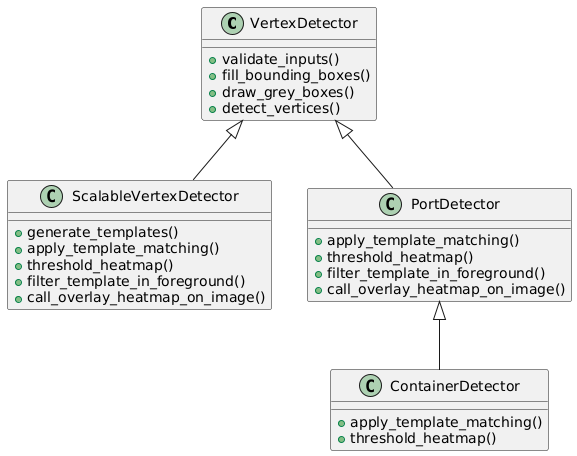
\includegraphics[width=0.5\textwidth]{pictures/inheritance_diagram.png}
    \caption[Inheritance diagram]{Inheritance diagram of the vertex detection classes created using \textit{PlantUML} \autocite{plantuml_2024}. The \textit{ContainerDetector} class inherits from the \textit{PortDetector} class, allowing it to reuse the majority of the functionality provided by \textit{PortDetector}.}
    \label{fig:inheritance_diagram}
\end{figure}
Depending on the vertex type, an object of either \textit{ScalableVertexDetector}, \textit{ContainerDetector} or \textit{PortDetector} is instantiated and used to detect the vertices.\\
The detected vertices are stored using a dedicated data storage function, ensuring subsequent steps proceed smoothly without requiring additional integration effort.

\section{Text Recognition Integration}
The integration of Easy\acrshort{ocr} into the \acrshort{xgee} codebase is achieved by utilizing the Easy\acrshort{ocr} \acrshort{api} within \textit{diagram\_tokenization\_orchestrator.py}. The \textit{detect\_text} function is updated to employ Easy\acrshort{ocr} for text extraction from preprocessed images. The extracted text is then stored using the existing dedicated data storage function, ensuring compatibility with subsequent processing steps.
Unlike PyTesseract, Easy\acrshort{ocr} includes inconsistent padding around detected text regions, resulting in less precise positional data. This discrepancy caused inconsistencies in positional accuracy and introduced errors in downstream model comparison methods. To ensure compatibility with the already existing interface, the dimensions of the bounding boxes were adjusted to more closely match those of PyTesseract. A positioning margin was implemented as well to reduce the need for bounding boxes to be positioned pixel-perfectly, reducing the amount of interfering error indications.

\section{Testing and Validation of the Integration}
To test the methods, the \acrshort{xgee} editor is used to create models with a known structure, incorporating different test cases in different editor layers. The model is processed by the verification pipeline. If necessary, text, vertex, or edge detections can be turned off to accelerate testing and reduce the workload when evaluating newly implemented methods. The results are compared to the expected output, and any discrepancies are analyzed to identify the cause. To further streamline the testing process, all previously mentioned methods log intermediate images and results using a dedicated Python logging package. This simplifies the process of identifying and resolving new issues.

To classify the performance of all newly implemented methods, 20 unique testcases in each editor model were processed and analyzed to demonstrate the functionality and limitations of the new additions. These evaluations are presented in \autoref{chap:evaluation}.